%% Template for SDP report, adapted from mlp_cw2_template, 2018. 

%% Based on  LaTeX template for ICML 2017 - example_paper.tex at 
%%  https://2017.icml.cc/Conferences/2017/StyleAuthorInstructions

\documentclass{article}
\usepackage[T1]{fontenc}
\usepackage{amssymb,amsmath}
\usepackage{txfonts}
\usepackage{microtype}
\usepackage{xspace}
\xspaceaddexceptions{\%}

% Lists with less spacing between items
\usepackage{paralist}

% For figures
\usepackage{graphicx}
\usepackage{subfig} 

% For citations
\usepackage{natbib}

% For algorithms
\usepackage{algorithm}
\usepackage{algorithmic}

% the hyperref package is used to produce hyperlinks in the
% resulting PDF.  If this breaks your system, please commend out the
% following usepackage line and replace \usepackage{mlp2017} with
% \usepackage[nohyperref]{mlp2017} below.
\usepackage{hyperref}
\usepackage{url}
\urlstyle{same}

% Packages hyperref and algorithmic misbehave sometimes.  We can fix
% this with the following command.
\newcommand{\theHalgorithm}{\arabic{algorithm}}


% Set up MLP coursework style (based on ICML style)
\usepackage{mlp2018}
\mlptitlerunning{SDP Demo \demoNumber  Group (\groupNumber)}
\bibliographystyle{icml2017}


\DeclareMathOperator{\softmax}{softmax}
\DeclareMathOperator{\sigmoid}{sigmoid}
\DeclareMathOperator{\sgn}{sgn}
\DeclareMathOperator{\relu}{relu}
\DeclareMathOperator{\lrelu}{lrelu}
\DeclareMathOperator{\elu}{elu}
\DeclareMathOperator{\selu}{selu}
\DeclareMathOperator{\maxout}{maxout}







%% You probably do not need to change anything above this comment

%% REPLACE the details in the following commands with your details
\setGroupNumber{18}
\setGroupName{Group 18}
\setProductName{Opticane}
\setDemoNumber{1}
\setLogoFileName{coollogo2.png}

\begin{document} 

\makeSDPTitle{Demo}

% Previous MLP Style Title Layout working. 
% \twocolumn[
    % \mlptitle{\productName: SDP Demo \demoNumber}
    % \centerline{Group \groupNumber: \groupName}
% ]

\begin{abstract} 
Our product is a device that can be added to a cane, like a sleeve, that helps visually impaired users navigate their surroundings by using lidar technology to detect nearby objects and providing haptic feedback. We now have a clear idea of what our project is going to be. For this demo we focused more on how we will use a LiDAR for our project and also discussed some advances we have made on the software part of our project. Another part of the demo will discuss the methods we will use to test our project. Lastly, we now have an estimate of how expensive our project will be.
\end{abstract} 


\section{Project plan update} 

Here are the goals we had for the first demo:
\begin{itemize}
    \item Have clear information about the device and how the mechanism works.[achieved]
    \item Have a LiDAR move around and collect data in an environment on Webots.[achieved]
    \item Know which LiDAR we would use for our project.[achieved]
    \item Decide on the type of tactile feedback the device would use.[achieved]
    \item Write this report describing our project.[achieved]

    
\end{itemize}


We used Trello to assign tasks to each member of the team and GitHub for integrating Lewis’s and Samuel’s code to have a Webots simulation to test the LiDAR in an environment.Table \ref{table 1} shows the individual work the team members have done for the demo and Figure \ref{figure 2} is a screenshot of the Trello board we are using to distribute work. Other than the work mentioned on Table \ref{table 1}, the group has met with Ryan Bowler on January 26th and Garry Ellard on January 27th to make modifications to our project.

After meeting with Ryan and doing more research, our group changed the project from a glove to a cane sleeve - a device which will be put over a cane's handle that will provide haptic feedback utilizing a mounted LiDAR's distance data. The sleeve will have a feature that will allow the user to adjust where the LiDAR detects objects.For more experienced cane users they can limit the detection to objects from the waist up and others can adjust it to detect objects on the ground as well. 

We have not used our budget this week other than meeting with Garry on Wednesday because we were finalizing the technicalities of the project. Going forward, for demo 2, we would like to demonstrate an array of LEDs reacting to our LiDAR's data both in simulation and in person, and would also like to have set up an initial draft of our website. For demo 3 we would like to be able to present a prototype of our tactile feedback system and integrate it into our website and simulation. Finally, for the final demo, we would like to have a polished website showcasing our product's performance both in-person and in simulation. Due to the pandemic, we expect to now have a fully complete hardware implementation, but want to at least have the core components 3D modeled and hopefully built.

\newblock
\section{Technical details}

The current implementation that we have in place for the first demo demonstrates our ability to utilize a LiDAR in simulation. As of now, to show that our project is feasible, we are establishing a solid foundation for testing both software and hardware. We are using a LiDAR as the main sensor in our product as it works well in low light conditions and helps us avoid computer vision algorithms. We considered echolocation/sonar or cameras but decided that those sensors incorporated much more software and hardware bandwidth than we were willing to spend.

We have shifted our product idea from a glove with haptic feedback to a sleeve that fits over a cane with haptic feedback. A sketch of what it should look like is shown on Figure \ref{figure 1}.With this shift, we would be able to keep the form factor of a cane, its use of indicating that the user is visually impaired, and additionally notify the user of objects in their vicinity through haptic feedback. In addition, we have decided to restrict the sensory feedback to ignore ground level objects as the cane itself solves that problem. 


\begin{figure}[hp!]
\begin{center}
  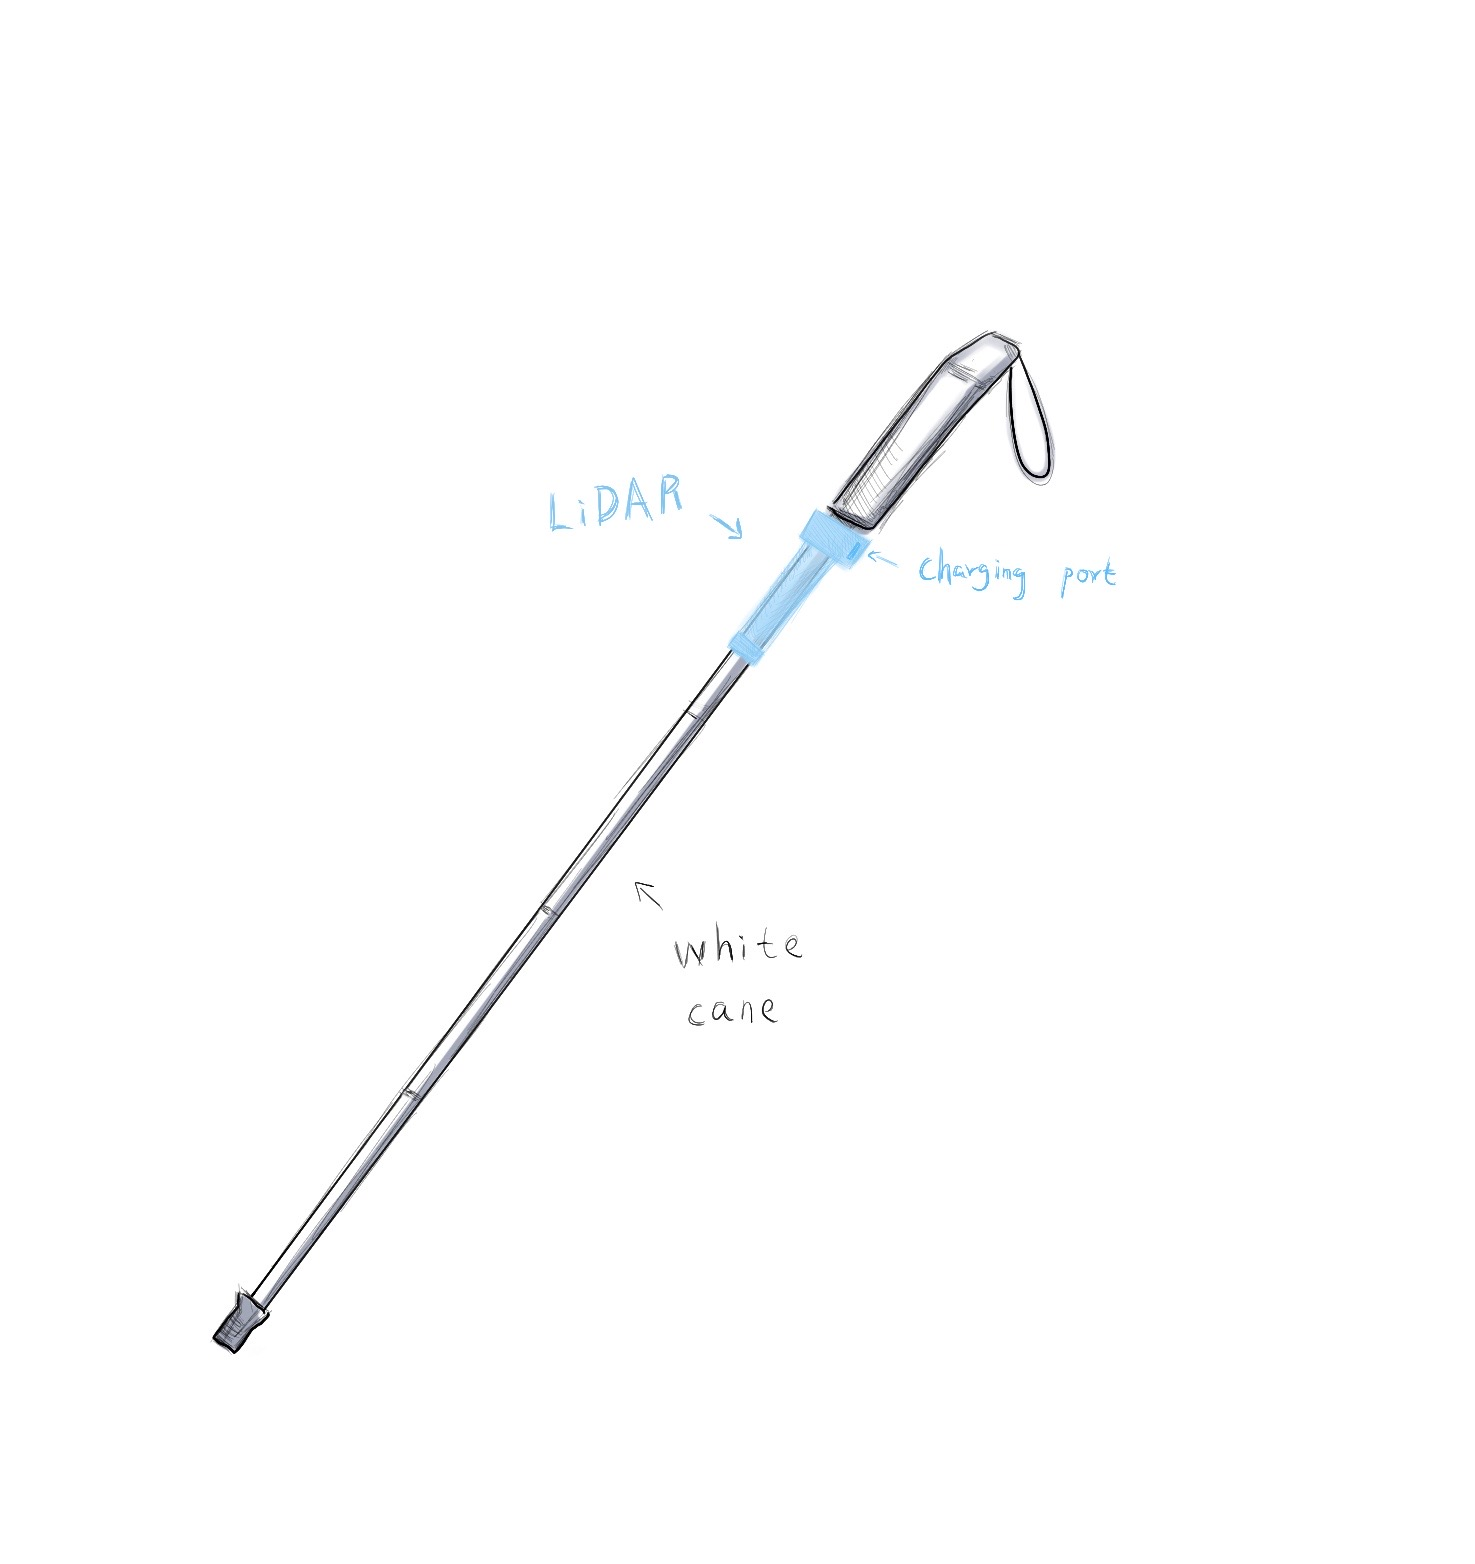
\includegraphics[width=0.5\textwidth,height=7cm]{cane2.png}
  \caption{Initial Product Sketch}
  \label{figure 1}
   \end{center}
\end{figure}

\begin{table*}[htbp!]
\vskip 3mm
\begin{center}
\begin{small}

\begin{tabular}{|l|l|}
\hline
Austin Pan  &  
    \begin{tabular}{l}
        \abovespace
        - Managed the team by assigning tasks to team members using Trello. \\
        - Held a class to discuss GitHub and Trello so everyone is comfortable with using it. \\
        - Worked on this report.
        \belowspace
    \end{tabular}  
\abovespace\belowspace \\
\hline
Ioana Buzduga & 
     \begin{tabular}{l}
        \abovespace
        - Worked on this report. \\
        - Made the Demo video.
        \belowspace
    \end{tabular} 
\abovespace\belowspace \\
\hline
Yuanting Mao & 
    \begin{tabular}{l}
        \abovespace
        - Researched different forms of tactile feedback and chose one that would best fit our project. 
        \belowspace
    \end{tabular} 
\abovespace\belowspace \\
\hline
Samuel Reves & 
    \begin{tabular}{l}
        \abovespace
        - Set up multiple testing environments in Webots to test the LiDAR including two apartment and a break room
        \belowspace
    \end{tabular} 
\abovespace\belowspace \\
\hline
Lewis Hamilton & 
    \begin{tabular}{l}
        \abovespace
        - Researched how to use a LiDAR in Webots.\\
        - Made a WeBots simulation showing the TurtleBot moving around and outputting data from the LiDAR
        \belowspace
    \end{tabular} 
\abovespace\belowspace \\
\hline
Shaoqing Zhao & 
    \begin{tabular}{l}
        \abovespace
        - Created an outline and a script for the Demo video.
        \belowspace
    \end{tabular} 
\abovespace\belowspace \\
\hline
Iman Abubakar & 
     \begin{tabular}{l}
        \abovespace
        - Helped manage the team by making sure everyone was on track.\\
        - Worked on this report.
        \belowspace
    \end{tabular} 
\abovespace\belowspace \\
\hline
Wazeed Naeem & 
    \begin{tabular}{l}
        \abovespace
        - Researched different types of LiDAR that we could use for our project.
        \belowspace
    \end{tabular} 
\abovespace\belowspace \\
\hline

\end{tabular}

\end{small}
\caption{Individual work of team members}
\label{table 1}
\end{center}
\vskip -3mm
\end{table*}

\begin{figure*}[htb!]
\begin{center}
  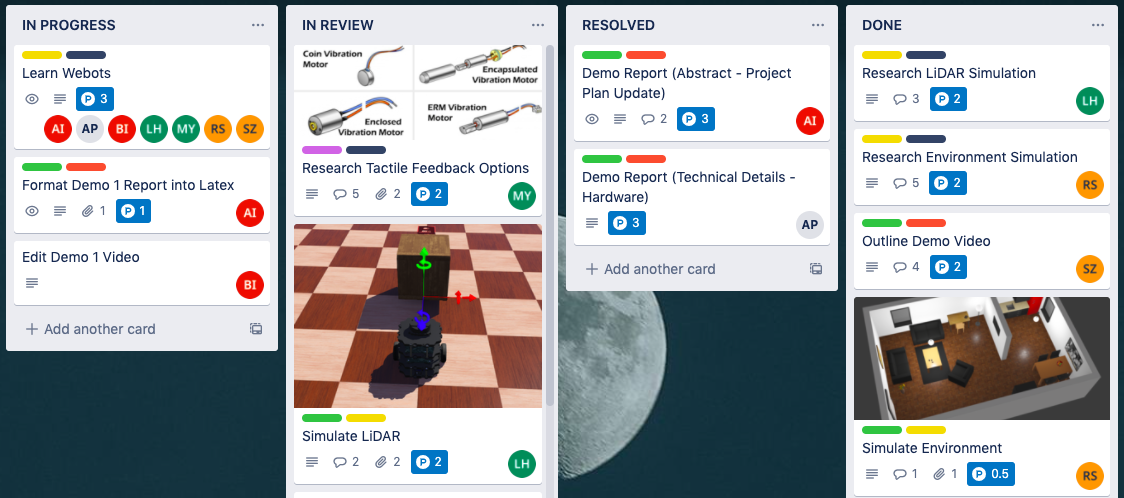
\includegraphics[width=1.01\textwidth,height=8cm]{Trello4.png}
  \caption{Screenshot of Trello board}
  \label{figure 2}
   \end{center}
\end{figure*}
\newpage
\subsection{ Hardware}
Due to the situation with distance learning, we haven't built anything yet. We have, however, begun to plan out initial hardware design choices that we would hopefully be able to work with. In terms of what we have planned so far, we have decided to work with the LDS-01 LiDAR found on the turtlebots. We chose to use a LiDAR instead of sonar and RFID because LiDARs are relatively cheap, provide accurate data in most conditions, and provide great range.
\newline
We have also decided on using vibration as a form of tactile feedback and using a DRV2605L motor for that. We considered eccentric rotation motors as well but ultimately chose DRV2605L because:

\begin{itemize}
    \item It's a Linear Resonant Actuator(LRA) - a type of motor that vibrates in one direction giving a more fine-grained feedback.
    \item It can give powerful vibrations.
    \item It’s programmable where we can program it ourselves or use a range of its built-in patterns.

    
\end{itemize}

\subsection{ Software}
Currently, we have set up a LiDAR in Webots simulation and gotten it to output distance data in Python. In addition, we have set up multiple test environments in simulation to test our product for the future. These test environments are Webots worlds that include a layout for an apartment, a breakroom, and a more furnished apartment than the first. With these, the foundation for our simulations has been solidified and testing code changes in the future has been simplified. In addition, because we can simulate the core portions of our product, it will hopefully be easily translated to an in-person product for testing.




\section{Evaluation}
This section will outline the testing methods used for our system and the results. It should be noted that we are still in the developing stage so we couldn’t test other parts of the device.


\subsection{Testing Methods}

Samuel simulated different environments where the LiDAR was tested. Those environments were: 

\begin{itemize}
    \item An apartment with a living room and kitchen.
   
    \item An apartment with one big living room, a kitchen, stairs and 2 bedrooms and 2 bathrooms.
     \item A break room similar to Appleton Tower Level 3. 
    
\end{itemize}

Our main goal for the first demo was  to set up the foundation parts of the simulation, there isn't that much functionality that we tested yet. The environments created will be useful for later stages of the project. 

\subsection{Test Results}
Lewis tested the  functionality of the simulation. The tests are present in Table \ref{table 2} . 

\section{Budget}
This section details the budget for the estimated total budget of our system. The budget is split into two categories:  Monetary and Technician Time. 

\subsection{Monetary}
After meeting with Garry on Wednesday, our group decided that we will need: 
\begin{itemize}
    \item A LiDAR in the Webots simulation environment that will cost around £130 ( \$179)  that will connect to the Turtlebot  already provided in Appleton Tower. For future demo videos Gary reckons that we would drive the turtlebot around the lab remotely, effectively acting like a proof of concept to our idea of a LiDAR attached to the middle of the cane  \cite{emanual} \cite{Cyberbotics} .  The budget for the LiDAR needs to be approved by Garry. 
    \item A raspberry pi that outputs to LEDs with different strengths rather than haptic feedback because haptic feedback is harder to demonstrate in videos. The raspberry pi is already provided as part of the course and we estimate a cost of £50.
    \item Vibration motor that costs around £50. The cost needs to be approved by Garry during the next meeting. 
    
\end{itemize}




\begin{table*}[h]
\vskip 3mm
\begin{center}

\begin{small}

\begin{tabular}{|p{8.32cm}|p{8.35cm}|}
\hline\hline
\abovespace\belowspace
Test & Result    \\
\hline\hline
\abovespace
Can LiDAR pick up wooden box in middle of its
view thereby outputting floats in the middle of the output list and not infs (which specify not object is
there)?
& The LiDAR accurately picks up float values for the box (albeit the simulated noise for the WeBots means there are deviations) in the middle of the list and outputs infs for the rest  
 \belowspace\\
\hline
\abovespace
Can the LiDAR pick up a variety of objects in the environment and can it detect more subtle objects such as gaps in the legs of the tables?
 & LiDAR picks up a variety of depth levels
corresponding to objects. What’s interesting is that if interpretations as correct the LiDAR picks up the gaps in the legs of tables as ‘inf’ values since those spaces are too deep for the LIDAR’s range
\belowspace \\
\hline
\abovespace
Given a cabinet that is ~2.5m away from the LiDAR in the simulation can the LiDAR to some degree of accuracy measure this distance and keep updating smaller and smaller distances as the LiDAR gets closer to the cabinet
& It does pick up values of around 2.5 and these values do decrease as the robot/LiDAR gets closer however there are lots of variations in the numbers around it, as the demo video shows. Therefore this test shows we must research/develop algorithms that allow us to recognise objects from depth values (particularly in accounting for variations in
depth one single object may have like test1 shows)
 \belowspace \\
\hline
\abovespace
We tested how the LiDAR would react and what data it would output to a long narrow corridor longer
 & While the LiDAR picked up accurate depth values
for objects left/right of the corridor, in the middle it
did seem to struggle picking up high (>3m) readings
and inf for the long ‘stretch’ of the corridor
\belowspace \\
\hline
\abovespace
How do different simulation environments affect runtime
 & While the software worked well for small
environments such as test 1,2 (~17Kb wbt files)
there was considerable slowdown for files around
~42 Kb while running the controller. This can be
seen in the slow execution speed of videos 3,4.
Optimisation of certain environments via through
use of sharing generic nodes may be needed
\belowspace \\
\hline


\end{tabular}

\end{small}
\caption{Test Results}
\label{table 2}

\end{center}

\vskip -3mm
\end{table*}

\begin{figure*}[hp!]
\begin{center}
  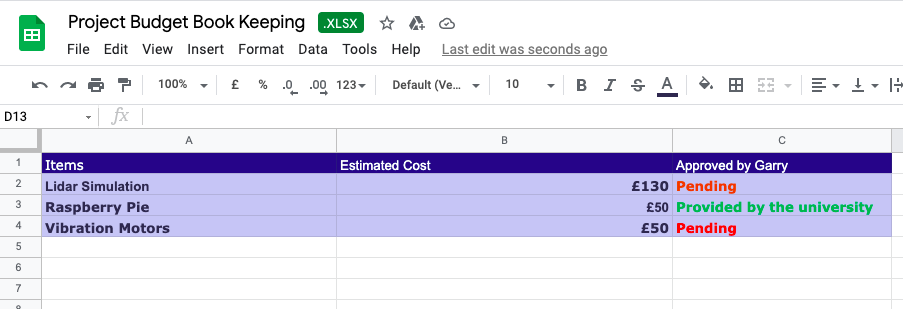
\includegraphics[width=1\textwidth,height=6cm]{cost.png}
  \caption{Screenshot of Project Budget Spreadsheet}
  \label{figure 3}
   \end{center}
\end{figure*}

Figure \ref{figure 3} shows a screenshot of a \href{https://docs.google.com/spreadsheets/d/1f9Xxwo_f1lgzSphoT1upxFMg0Z1Rc181/edit#gid=1746507455}{spreadsheet} that shows the project budget of everything we used for our system, including the ones already provided by the university. The budget will be updated weekly by Iman, the Head of Hardware Leader and Co-Product Manager. The spreadsheet will be shared with Garry, after the meeting happening next week. 


\subsection{Technician Time }
The group decided to use 1 hour per week to meet with the technicians. The meetings will be scheduled prior that week. The Head of Hardware Team (Iman) will be in charge of arranging a meeting with the technician every week and discuss the technicalities of the system. Everyone from the team is welcomed to attend the meeting, but the priorities should be Iman and Wazeed as they are part of the hardware team and Austin as Co-Product Manager and Head of Software Team, because it is important to know how to make the connection between the software and hardware. 

\section{Video}
The demo video can be found  \href{https://uoe.sharepoint.com/:v:/s/SDP2021-Group-18_/EVqoBITskpBPu1HTftugXQsBEp29XuYYGY-UFZv7lIEHww?e=iEbhEi}{here}.
%% Include any references in a bibliography

\bibliography{example-refs}

\end{document} 
